% paper/joss/architecture.tex -- the engine-architecture figure of the JOSS
% paper (architecture.png): a standalone copy of Figure fig:arch of
% paper/whitepaper/whitepaper.tex, with one label moved off an arrow.
% Prose and figure: CC BY-SA 4.0.  Rebuild (from this directory):
%   pdflatex architecture.tex
%   pdftoppm -png -r 220 -singlefile architecture.pdf architecture
\documentclass[border=6pt]{standalone}
\usepackage[T1]{fontenc}
\usepackage[utf8]{inputenc}
\usepackage{lmodern}
\usepackage{xcolor}
\usepackage{tikz}
\usetikzlibrary{positioning,fit,arrows.meta,calc}
\definecolor{linkink}{RGB}{20,60,110}
\begin{document}
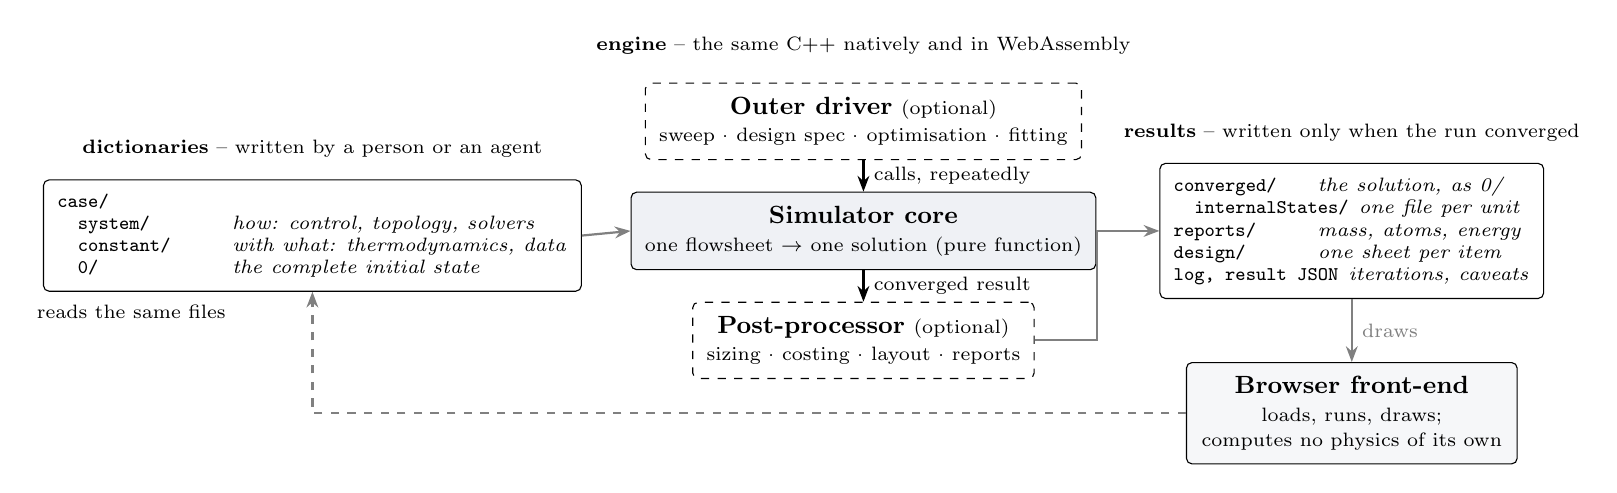
\begin{tikzpicture}[
    box/.style={draw, rounded corners=2pt, align=center, font=\small,
                inner sep=5pt},
    lay/.style={box, minimum width=4.2cm, minimum height=0.85cm},
    opt/.style={lay, dashed},
    arr/.style={-{Stealth[length=2mm]}, thick},
    node distance=0.4cm]
  % the dictionaries
  \node[draw, rounded corners=2pt, align=left, font=\scriptsize\ttfamily,
        inner sep=5pt] (case) {%
    case/\\
    \ \ system/\ \ \ \ \ \ \ \ \textrm{\itshape how: control, topology, solvers}\\
    \ \ constant/\ \ \ \ \ \ \textrm{\itshape with what: thermodynamics, data}\\
    \ \ 0/\ \ \ \ \ \ \ \ \ \ \ \ \ \textrm{\itshape the complete initial state}};
  \node[font=\scriptsize, align=center, above=0.15cm of case]
    {\textbf{dictionaries} -- written by a person or an agent};
  % the engine
  \node[opt, right=0.8cm of case, yshift=1.45cm] (outer)
    {\textbf{Outer driver} \scriptsize(optional)\\[-1pt]
     \scriptsize sweep · design spec · optimisation · fitting};
  \node[lay, below=of outer, fill=linkink!7] (core)
    {\textbf{Simulator core}\\[-1pt]
     \scriptsize one flowsheet $\rightarrow$ one solution (pure function)};
  \node[opt, below=of core] (post)
    {\textbf{Post-processor} \scriptsize(optional)\\[-1pt]
     \scriptsize sizing · costing · layout · reports};
  \draw[arr] (outer) -- node[right, font=\scriptsize]{calls, repeatedly} (core);
  \draw[arr] (core) -- node[right, font=\scriptsize]{converged result} (post);
  \node[draw=none, fit=(outer)(core)(post), inner sep=6pt] (engine) {};
  \node[font=\scriptsize, align=center, above=0.02cm of engine]
    {\textbf{engine} -- the same C++ natively and in WebAssembly};
  \draw[arr, gray] (case.east) -- (core.west);
  % the results
  \node[draw, rounded corners=2pt, align=left, font=\scriptsize\ttfamily,
        inner sep=5pt, right=0.8cm of core] (res) {%
    converged/\ \ \ \ \textrm{\itshape the solution, as 0/}\\
    \ \ internalStates/\ \textrm{\itshape one file per unit}\\
    reports/\ \ \ \ \ \ \textrm{\itshape mass, atoms, energy}\\
    design/\ \ \ \ \ \ \ \textrm{\itshape one sheet per item}\\
    log, result JSON\ \textrm{\itshape iterations, caveats}};
  \node[font=\scriptsize, align=center, above=0.15cm of res]
    {\textbf{results} -- written only when the run converged};
  \draw[arr, gray] (post.east) -| ($(post.east)!0.5!(res.west)$) |- (res.west);
  % the GUI
  \node[box, below=0.8cm of res, minimum width=4.2cm, fill=linkink!4] (gui)
    {\textbf{Browser front-end}\\[-1pt]
     \scriptsize loads, runs, draws;\\[-2pt]
     \scriptsize computes no physics of its own};
  \draw[arr, gray] (res.south) -- node[right, font=\scriptsize]{draws} (gui.north);
  \draw[arr, gray, dashed] (gui.west) -| ($(case.south)+(0,-0.3)$) -- (case.south);
  \node[font=\scriptsize, below=0.05cm of case, xshift=-2.3cm, align=center]
    {reads the same files};
\end{tikzpicture}
\end{document}
